%%%%%%%%%%% DTI report %%%%%%%%%%%
\documentclass[a4paper,11pt,oneside]{DTI}

% *************** Load packages ***************
\usepackage[T1]{fontenc}
\usepackage[italian]{babel}
\usepackage{graphicx}
\usepackage{url}
\usepackage{subfigure}
\usepackage{makeidx}
\usepackage[utf8]{inputenc}
\usepackage{booktabs}
\usepackage[colorlinks]{hyperref}
\usepackage{amsmath}
\usepackage{amsfonts}
\usepackage{amssymb}
\usepackage{float}
\usepackage{listings}

\title{Traveling Salesman Problem}
\subTitle{19\ap{a} Coppa di Algoritmi} 
\author{Filippo Pura}

\date{\today}

\lstset{language=bash}

% Crea un capitolo senza numerazione che per� appare nell'indice %
\newcommand{\problemchapter}[1]{%
  \chapter*{#1}%
  \addcontentsline{toc}{chapter}{#1}%
\markright{#1}{}}

%*****************************************************************

% Numerazione delle appendici secondo norma %
\addto\appendix{\renewcommand{\thesection}{\Alph{section}} 
\renewcommand{\thesubsection}{\thesection.\arabic{subsection}}}
%*****************************************************************

\makeindex % Crea l'indice analitico, se è necessario scommentarlo
\begin{document}
\maketitle
\frontmatter
\newpage
\mainmatter
% *************** Main matter ***************
\chapter*{Problema}
\label{cha_problema}

Il problema del commesso viaggiatore consiste nella ricerca del ciclo hamiltoniano più breve all'interno di un grafo pesato completo. Questo tipo di problema appartiene alla classe dei problemi \emph{NP-Completi}. In Figura~\ref{fig_eil76} è mostrato uno dei problemi TSP con soluzione, sottoinsieme dei problemi NP.

\begin{figure}[H]
  \centering
  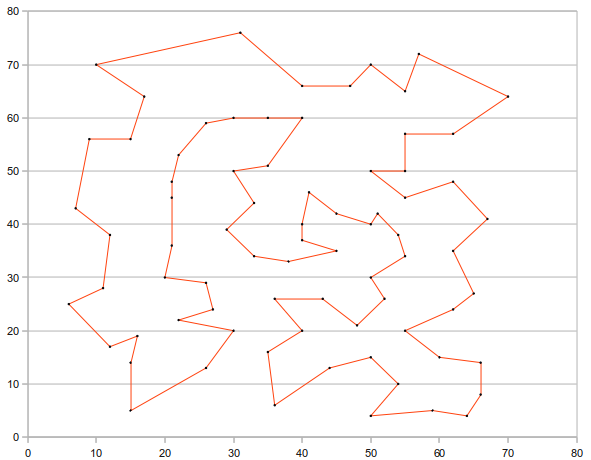
\includegraphics[width=10.0cm]{immagini/eil76.png}
  \caption{Eil76, problema di TSP da 76 città\label{fig_eil76}}
\end{figure}

Il compito assegnato è di generare una soluzione ammissibile e quanto più possibile vicina a quella ottimale (ovvero la migliore) in 3 minuti di esecuzione del programma. Il programma deve poter lavorare su 10 problemi diversi:
\begin{itemize}
  \item \emph{ch130};
  \item \emph{d198};
  \item \emph{eil76};
  \item \emph{fl1577};
  \item \emph{kroA100};
  \item \emph{lin318};
  \item \emph{pcb442};
  \item \emph{pr439};
  \item \emph{rat783};
  \item \emph{u1060}.
\end{itemize}


\chapter*{Soluzioni implementate}
\label{cha_soluzioni}

\section*{Algoritmo costruttivo}
\label{sec_costruttivo}
È stato utilizzato un algoritmo Nearest Neighbour per comporre una soluzione da cui poter derivare
il suo costo ed impostare di conseguenza il feromone iniziale degli archi usati per l'algoritmo 
Ant Colony System.\newline
Esso è eseguito solo una volta, all'inizio dell'esecuzione sul set di città ricavate dal file.\newline
Similarmente viene usata un'implementazione dell'algoritmo di Kruskal per comporre il Minimum Spanning
Tree, esso viene poi utilizzato per comporre le candidate lists di ogni città, ovvero tutte le città direttamente
collegate ad essa nel Minimum Spanning Tree più un numero variabile di città più vicine non considerando quelle 
inserite precedentemente.
\noindent 

\section*{Algoritmi di ottimizzazione locale}
\label{sec_ottimizzazione}
Come ottimizzazione locale ho implementato l'algoritmo Two Opt usando le candidate lists ed un array di
supporto per trovare in modo rapido gli indici delle città nel percorso.\newline
Esso è generato contemporaneamente al percorso nell'algoritmo Ant Colony System.\newline
Il ciclo esterno definisce l'indice 'i', il cui itera da 0 fino alla lunghezza del percorso.\newline
L'indice 'j' viene derivato dalla posizione nel percorso delle città presenti nella candidate list della città 
specificata dall'indice 'i'.\newline
Dopo il completamento del ciclo 'i' esterno si effettua lo scambio con gli indici dai quali si è calcolato
il guadagno migliore. \newline
L'algoritmo si ripete fintanto che nessun guadagno viene trovato dopo un'iterazione completa.

\section*{Algoritmi meta-euristici}
\label{sec_metaeuristici}
L'algoritmo principale del progetto è composto da un'implementazione leggermente più "greedy" dell'Ant 
Colony System. \newline
Questo perché in modalità di esplorazione viene comunque considerata la "best choice" ovvero la città
con più probabilità di venire scelta determinata dalla distanza e dal feromone del suo arco.\newline
Come parametro del feromone iniziale uso \textit{1/(C(percorso generato dal Nearest Neighbour) * Numero di città)}.\newline
Come opzione di movimento delle formiche ad ogni avanzamento considero soltanto le città presenti nella candidate list
della città corrente, nel caso in cui tutte le città presenti in essa siano già state
visitate viene selezionata la città non visitata più vicina a quella corrente. \newline
Dopo aver eseguito una mossa, decremento il feromone dell'arco percorso secondo la formula dell'aggiornamento locale.\newline
Ogni volta che una formica termina un percorso, prima di eseguire ulteriori controlli, ottimizzo e sostituisco
il percorso ottenuto dalla formica tramite l'algoritmo Two Opt. \newline
L'aggiornamento globale del feromone viene applicato dopo ogni iterazione dell'algortimo, su tutti gli archi del percorso migliore assoluto.


\chapter*{Esecuzione programma}
\label{cha_esecuzione}

\section*{Piattaforma}
\label{sec_piattaforma}
La piattaforma usata è un computer portatile Aspire V3 - 772G. Nella Tabella~\ref{tab_statpc} sono mostrati alcuni parametri rilevanti.

\begin{table}[htb]
  \caption{Plattaforma usata per i test\label{tab_statpc}}
  \centering
\begin{tabular}{ll}
  \toprule
  Sistema Operativo		& Windows 8.1 \\
  Processore			& Intel Core i7 4702MQ @ 2.2GHz \\
  RAM				& 32GB \\
  \bottomrule
\end{tabular}
\end{table}

\section*{Compilazione ed esecuzione}
\label{sec_comp_exec}
Per eseguire l'algoritmo su ogni problema fornito è sufficente eseguire il comando mvn:test.
Ogni istanza di test avvia il programma principale passando come parametri il percorso per i 
file input necessari (seed più parametri e informazioni del problema) e il percorso dove salvare
il file di output del percorso trovato. \\
Ogni test è limitato a 3 minuti con un secndo di scarto. \\
Per ogni problema viene anche mostrato su terminale lo stato attuale dell'algoritmo sotto 
forma di costo del percorso quando esso viene migliorato e un output finale con il tempo 
mancante allo scadere dei 3 minuti da quando è stata trovata l'ultima soluzione migliore.



\chapter*{Framework per run automatizzate}
\label{cha_framework}

Per eseguire le test runs non è stato utilizzato nessun framework esterno. \\
La ricerca dei seed è stata effettuata con un semplice metodo di test il quale instanzia 
l'applicazione principale usando parametri casuali che vengono salvati in un apposito file
\emph{.seed} nel caso in cui il percorso ottenuto sia migliore di tutti quelli trovati 
precedentemente.
\chapter*{Risultati}
\label{cha_risultati}

In Tabella~\ref{tab_migliori} sono mostrati i risultati migliori per ogni problema. 
Nella cartella \emph{final} sono presenti tutti i file \emph{.seed} usati per trovare
questi risultati. Nella cartella \emph{optTours} sono riportati i relativi file \emph{.opt.tour}.
I tour risultanti vengono salvati sotto \emph{final/\{problemname\}}.
\begin{table}[htb]
  \caption{Soluzioni we migliori per ogni problema}
  \label{tab_migliori}
  \centering
\begin{tabular}{lrrrr}
  \toprule
  Problema		&	Optimum		&	Risultato	&	Errore		&	Seed files		\\
  \midrule
  ch130			&	6110		&	6110		&	0\%	&	ch130.seed	\\
  d198			&	15780		&	15780		&	0\%	&	d198.seed	\\
  eil76			&	538		&	538		&	0\%	&	eil76.seed	\\
  fl1577		&	22249		&	22408		&	0.7095\%	&	fl1577.seed	\\
  kroA100		&	21282		&	21282		&	0\%	&	kroA100.seed	\\
  lin318		&	42029		&	42029		&	0\%	&	lin318.seed	\\
  pcb442		&	50788		&	50788		&	0\%	&	pcb442.seed	\\
  pr439			&	107217		&	107217		&	0\%	&	pr439.seed	\\
  rat783		&	8806		&	8808		&	0.0227\%	&	rat783.seed	\\
  u1060			&	224094		&	224515		&	0.1875\%	&	u1060.seed	\\
  \midrule
  media			&			&			&	0.0919\% 	&			\\
  \bottomrule
\end{tabular}
\end{table}

\chapter*{Conclusioni}
\label{cha_conclusioni}

L'algoritmo implementato è particolarmente efficente ma mancano dei piccoli particolari e accorgimenti necessari 
per velocizzare ulteriormente il processo e raggiungere così lo 0\% su tutti i file.
Uno di questi potrebbe essere l'implementazione dei Don't Look Bits all'interno dell'algortimo Two
Opt oppure una scelta più accurata e/o dinamica delle candidate lists delle città. \\
Per concludere ho trovato l'esperienza e l'approccio per questo progetto molto divertente e piacevole. 
\end{document}
